
\documentclass[runningheads]{llncs}

\usepackage{amssymb}
\usepackage[english]{babel}
\usepackage[utf8]{inputenc}
\setcounter{tocdepth}{3}
\usepackage{graphicx}

\usepackage{url}
\urldef{\mailsa}\path|{jrra,ksma,atka}@itu.dk|
\newcommand{\keywords}[1]{\par\addvspace\baselineskip
\noindent\keywordname\enspace\ignorespaces#1}
\graphicspath{{images/}}

\begin{document}

\mainmatter  % start of an individual contribution

% first the title is needed
\title{Model-Driven Development Project:\\ Modelling, Domain-Specific Language\\ and Code Generation}

% a short form should be given in case it is too long for the running head
\titlerunning{Model-Driven Development Project}

\author{Jacob Romme Rasmussen \and \\ Kristian Støving Mørk Andersen \and \\ Athanasios Kastanidis}
%
\authorrunning{Model-Driven Development Project}

\institute{\mailsa\\}

\toctitle{Lecture Notes in Computer Science}
\tocauthor{Authors' Instructions}
\maketitle


\begin{abstract}
This paper covers the process of modelling and structuring an external domain-specific language with the sole purpose of writing surveys. The language comes with its own editor and compiler. Code is automatically generated from the constructed surveys and targets multiple platforms, namely the Android mobile platform and a web platform. 
\keywords{Model-driven development, Meta-model, DSL, Code generation, Android, HTML}
\end{abstract}

\section{Introduction}

What is the purpose of this project?
Objectives? Goals? What do you want to achieve?
What are the benefits(and disadvantages\/cost) of using a domain
specific language for this task?
What are the requirements for your DSL? Who is the target user?
How much you have managed to achieve?

\section{System Overview}
\begin{figure}
\centering
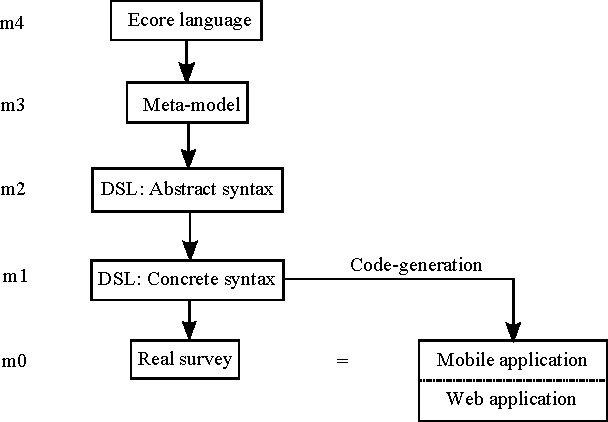
\includegraphics[height=6.2cm]{modelhierarchy}
\caption{A figure depicting the model hierarchy of the system. The m-levels are an inspiration by the Meta-Object Facility (MOF)\textbf{CITE}.}
\label{fig:mhier}
\end{figure}

\section{Language Design}
Domain analysis and the meta-model
Concrete-syntax (interesting aspects of the grammar)
How and what design principles you followed? (cite literature) \\
When performing the domain analysis we searched for the most popular online survey sites and chose to use the survey templates provided by Surveymonkey\cite{surveymonkey} and Obsurvey\cite{obsurvey} as inspiration. The language is specifically designed to support their survey design. The surveys span a variety of different types of questions. Multiple answers can be given to some questions, while others only allow a single answer. Most answers are preset, while some allows the user to type free text. A question can contain answers of both types. The questions are either listed on a single page or divided into several pages. A question can depend on previous answers meaning it is only shown if a certain answer was chosen earlier. This is useful when some answers make the following questions irrelevant. The combined functionality of the investigated surveys lead to the following requirements for the survey system:
\begin{itemize}
\item  A survey must contain at least one question. 
\item A question has a type indicating the amount and types of answers allowed. 
\item A question can require specific previous answers and should only be made available if all the required answers were chosen by the user. 
\item Multiple choice questions allow users to choose multiple predefined answers.
\item RadioChoice questions should only allow a single answer. 
\item Open questions do not contain any predefined answers but allow a user to define the answer themselves. 
\item An open question must contain a single answer.
\end{itemize}
The structure of the meta-model shown in figure \ref{??} is based on these requirements and as such attempts to capture the structure of the investigated surveys. The Survey root element contains one or more questions. The question entity is split into three subentities denoting the type of question. An alternative approach would be to merge the MultipleChoice and RadioChoice entities and use an enumeration to describe a question type attribute. However, we argue that it is visually more pleasing to have the distinct separation displayed in the model. A question contains one or more references to answers denoting the relevancy of the question. A constraint is run on the model checking that no question requires one of its own answers. The model provides the basis for the abstract syntax of the domain-specific language, which is used to write a survey in concrete syntax.   
\medskip

\noindent
{\it Example of the concrete syntax in a <MySurvey>.survey-file is shown below}
\begin{verbatim}
multiple:
	"What is your favourite pet?"
	answer dogAnswer "Dogs"
	text otherAnswer "Something else?"

single:
	"Which is better - Coffee or tea?"
	optional
	requires dogAnswer
	answer teaAnswer "Tea"
	answer coffeeAnswer "Coffee" 

open:
	"Describe how you feel about Windows XP."
	optional
	text xpAnswer
\end{verbatim}
%
\noindent
A .survey file contains one or more question-segments. A segment defines the type of the question followed by a surveyor-defined description - the actual question to be read by the surveyee. The optional-keyword is used to indicate if the question in the given segment is optional. The remainder of the segment contains a list of answers starting with the answer-keyword, followed by an identifier and a description (the actual predefined answer). The identifier is only used internally when referencing the answer from somewhere else in the file. The referencing of answers is used when \emph{requiring} that certain answers have been chosen by the surveyee in order for the question to be relevant. The naming of the keywords are chosen specifically to capture the essence of their functionality and be easily understandable by anyone with no prior programming experience or the like. Since many of the keywords are names of concepts used in the survey domain, the intention is that only minor knowledge about surveys is enough to be able to use the DSL with ease. 

\section{Architecture of the language implementation}
Internal\/External DSL? Interpreted? Generating code? Use of
model-to-model transformations?
Reuse between different back-ends? Coupling between back-ends and
between the front-end and the back-ends?
Toolchain elements? What tools do you provide? What tools one could
provide as an extension?
Cogen argument about advantages of your architecture, maintainability,
development cost.
Are the requirements met?
How did you test the implementation?

\begin{thebibliography}{4}

\bibitem{jour} Smith, T.F., Waterman, M.S.: Identification of Common Molecular
Subsequences. J. Mol. Biol. 147, 195--197 (1981)

\bibitem{book} Foster, I., Kesselman, C.: The Grid: Blueprint for a New Computing
Infrastructure. Morgan Kaufmann, San Francisco (1999)

\bibitem{proceeding1} Czajkowski, K., Fitzgerald, S., Foster, I., Kesselman, C.: Grid
Information Services for Distributed Resource Sharing. In: 10th IEEE
International Symposium on High Performance Distributed Computing, pp.
181--184. IEEE Press, New York (2001)

\bibitem{surveymonkey}SurveyMonkey, \url{http://www.surveymonkey.com/s/Public-School-Survey-Template}

\bibitem{obsurvey}Obsurvey, \url{http://www.obsurvey.com/language-proficiency-template/}

\end{thebibliography}

\end{document}
